\chapter{Introdução}\label{CAP:introducao}

Este documento detalha a concepção e implementação de um sistema dedicado à aquisição e análise de dados relacionados à condução de um motorista.

A abordagem central consiste na extração de informações provenientes de sensores já presentes em veículos contemporâneos, acessando a porta OBD-II, que adota um padrão internacional para o diagnóstico de parâmetros internos de um automóvel\textsuperscript{[2]}.

Adicionalmente, são coletadas informações fornecidas por um dispositivo móvel, incluindo dados de geolocalização e acelerômetros, e essas informações são centralizadas em uma base de dados hospedada na AWS. 

Esta arquitetura permite uma análise posterior aprofundada desses dados, promovendo \textit{insights} valiosos sobre os padrões e comportamentos de direção.

\section{Motivação}

Buscando traçar o perfil de condução de um motorista e desenvolver uma categorização clara para os condutores, este projeto empenha-se na criação de uma infraestrutura dedicada à captação e análise de dados em veículos de uso pessoal.

Com base nos dados de aceleração, é possível classificar o estilo de direção, identificar comportamentos potencialmente perigosos no trânsito e antecipar a necessidade de manutenção do veículo. Ao integrar a análise dos dados ao sistema de perfilamento, não apenas contribui-se para a segurança do veículo, mas também viabiliza-se a personalização de \textit{feedbacks} e sugestões ao condutor, promovendo uma condução mais eficaz e segura.

Uma investigação preliminar sobre o tema revelou a existência de uma patente para um produto semelhante, registrada em 2013, que avalia o desempenho do motorista a partir de dados previamente coletados de parâmetros relevantes à condução do veículo\textsuperscript{[1]}.


\section{Objetivo}

Este trabalho procura criar uma plataforma de disponibilização e captura de dados em um carro, coletando as informações \textit{in loco} e apresentando estatísticas relevantes derivadas do que foi coletado.

Para isso, foi feito uso da infraestrutura já presente em carros atuais. Conforme pode ser visto na imagem \ref{fig:sensors_car}, alguns carros podem ter dezenas de sensores embarcados dentro de si.


\begin{figure}[hp]
    \centering
    
    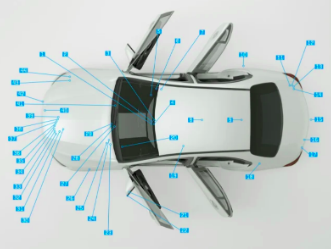
\includegraphics[]{figures/sensores_carro.png}
    
    \caption{Veículos modernos estão equipados com dezenas de sensores\textsuperscript{[2]}.}
    
    \label{fig:sensors_car}
\end{figure}

Essas informações foram complementadas com o uso de um \textit{smartphone}, o qual disponibiliza outros tipos de dados graças a seus sensores embarcados e à sua conexão com os satélites de GPS.

A análise da aceleração desempenha um papel essencial na avaliação do comportamento do motorista em sistemas de coleta de dados. Ao monitorar os padrões de aceleração, é possível extrair informações valiosas sobre a condução, tais como a suavidade nas transições de velocidade, a resposta a alterações nas condições de tráfego e o nível de agressividade ao volante.

A aceleração é um parâmetro que revela a habilidade do motorista em manter uma condução estável e antecipar suas ações em situações específicas. 

Por isso, a fase de análise dos dados coletados deste projeto focou em analisar esta grandeza física para perfilar a direção de um motorista.

O trabalho também utilizou dados de violência no Brasil para contribuir com a classificação do que seria "dirigir com segurança".

% Esse entendimento contribui para a compreensão do estilo de direção de cada condutor. 

% A maior parte da coleta de dados foi feita em um Hyundai Ix35, e dados estáticos foram tomadas de outros modelos também (Mercedes-Benz C200, Ford EcoSport e Volkswagen Saveiro) para conferência de parâmetros disponibilizados em comum por veículos de marcas diferentes.

Uma possível aplicação desse sistema encontra-se na área das empresas de seguro automotivo. Os dados e análises disponibilizados pelo aplicativo podem ser empregados na elaboração de políticas de precificação de seguros de veículos. 

Essa abordagem oferece a possibilidade de estabelecer um preço mais personalizado e justo para cada indivíduo, promovendo, assim, comportamentos mais responsáveis no trânsito. 

% Essa iniciativa não apenas contribui para a equidade na precificação, mas também estimula práticas de condução mais seguras e conscientes.

 
\section{Justificativa}
% ROMEO e PIRES [GIT]
% Pq o trabalho é importante?
No ano de 2021, 11.647 pessoas perderam a vida em acidentes de trânsito no Brasil\textsuperscript{[6]}. Além disso, a nível global, a média anual de fatalidades no trânsito atinge 1,35 milhão de pessoas\textsuperscript{[7]}, um número comparável às mortes por Covid-19 até abril de 2022\textsuperscript{[8]}.

Diante desses dados alarmantes, a importância deste projeto torna-se evidente, uma vez que estabelece métricas significativas para a avaliação do comportamento dos motoristas. Essas métricas não apenas contribuem para a prevenção de acidentes, mas, sobretudo, para a preservação da vida humana. O projeto emerge como uma ferramenta valiosa na promoção da segurança nas ruas e na busca por soluções que possam mitigar essas estatísticas trágicas.

Os veículos autônomos estão rapidamente conquistando popularidade, de forma que eles tornarem-se a maioria nas estradas é uma realidade iminente. Prevê-se, de fato, que carros com pelo menos nível 4 de automação tornem-se mais comuns a partir de 2025\textsuperscript{[9]}.

Dessa forma, embora a influência humana possa perder relevância em acidentes do futuro, torna-se imperativo estabelecer métricas para avaliar a condução de veículos autônomos. 

Essa abordagem é essencial para assegurar a segurança e eficiência desses automóveis, promovendo um padrão consistente de avaliação que contribua para a confiança generalizada no crescente uso de tecnologias autônomas.

Este projeto tem, portanto, extrema relevância, pois é uma possível ferramenta para reduzir as fatalidades no trânsito, independentemente de serem causadas por condutores humanos ou por veículos autônomos.

\section{Organização do trabalho}
Os próximos capítulos explicitarão como o trabalho foi planejado a partir de seus requisitos e das tecnologias envolvidas.

O projeto consistiu em integrar a porta OBD-II de qualquer carro com a plataforma de armazenamento de dados que foi criada.

Para isso, o Capítulo 2 faz uma breve apresentação dos conceitos usados neste projeto. O Capítulo 3, por sua vez, traz as etapas de desenvolvimento do trabalho e o Capítulo 4 mostra quais requisitos foram definidos para o sistema. Além disso, o desenvolvimento inicial do trabalho é descrito no Capítulo 5. Por último, o Capítulo 6 traz as considerações finais com uma breve discussão das conclusões do trabalho, assim como contribuições e sugestões para a continuidade dele.